\documentclass[1p]{elsarticle_modified}
%\bibliographystyle{elsarticle-num}

%\usepackage[colorlinks]{hyperref}
%\usepackage{abbrmath_seonhwa} %\Abb, \Ascr, \Acal ,\Abf, \Afrak
\usepackage{amsfonts}
\usepackage{amssymb}
\usepackage{amsmath}
\usepackage{amsthm}
\usepackage{scalefnt}
\usepackage{amsbsy}
\usepackage{kotex}
\usepackage{caption}
\usepackage{subfig}
\usepackage{color}
\usepackage{graphicx}
\usepackage{xcolor} %% white, black, red, green, blue, cyan, magenta, yellow
\usepackage{float}
\usepackage{setspace}
\usepackage{hyperref}

\usepackage{tikz}
\usetikzlibrary{arrows}

\usepackage{multirow}
\usepackage{array} % fixed length table
\usepackage{hhline}

%%%%%%%%%%%%%%%%%%%%%
\makeatletter
\renewcommand*\env@matrix[1][\arraystretch]{%
	\edef\arraystretch{#1}%
	\hskip -\arraycolsep
	\let\@ifnextchar\new@ifnextchar
	\array{*\c@MaxMatrixCols c}}
\makeatother %https://tex.stackexchange.com/questions/14071/how-can-i-increase-the-line-spacing-in-a-matrix
%%%%%%%%%%%%%%%

\usepackage[normalem]{ulem}

\newcommand{\msout}[1]{\ifmmode\text{\sout{\ensuremath{#1}}}\else\sout{#1}\fi}
%SOURCE: \msout is \stkout macro in https://tex.stackexchange.com/questions/20609/strikeout-in-math-mode

\newcommand{\cancel}[1]{
	\ifmmode
	{\color{red}\msout{#1}}
	\else
	{\color{red}\sout{#1}}
	\fi
}

\newcommand{\add}[1]{
	{\color{blue}\uwave{#1}}
}

\newcommand{\replace}[2]{
	\ifmmode
	{\color{red}\msout{#1}}{\color{blue}\uwave{#2}}
	\else
	{\color{red}\sout{#1}}{\color{blue}\uwave{#2}}
	\fi
}

\newcommand{\Sol}{\mathcal{S}} %segment
\newcommand{\D}{D} %diagram
\newcommand{\A}{\mathcal{A}} %arc


%%%%%%%%%%%%%%%%%%%%%%%%%%%%%5 test

\def\sl{\operatorname{\textup{SL}}(2,\Cbb)}
\def\psl{\operatorname{\textup{PSL}}(2,\Cbb)}
\def\quan{\mkern 1mu \triangleright \mkern 1mu}

\theoremstyle{definition}
\newtheorem{thm}{Theorem}[section]
\newtheorem{prop}[thm]{Proposition}
\newtheorem{lem}[thm]{Lemma}
\newtheorem{ques}[thm]{Question}
\newtheorem{cor}[thm]{Corollary}
\newtheorem{defn}[thm]{Definition}
\newtheorem{exam}[thm]{Example}
\newtheorem{rmk}[thm]{Remark}
\newtheorem{alg}[thm]{Algorithm}

\newcommand{\I}{\sqrt{-1}}
\begin{document}

%\begin{frontmatter}
%
%\title{Boundary parabolic representations of knots up to 8 crossings}
%
%%% Group authors per affiliation:
%\author{Yunhi Cho} 
%\address{Department of Mathematics, University of Seoul, Seoul, Korea}
%\ead{yhcho@uos.ac.kr}
%
%
%\author{Seonhwa Kim} %\fnref{s_kim}}
%\address{Center for Geometry and Physics, Institute for Basic Science, Pohang, 37673, Korea}
%\ead{ryeona17@ibs.re.kr}
%
%\author{Hyuk Kim}
%\address{Department of Mathematical Sciences, Seoul National University, Seoul 08826, Korea}
%\ead{hyukkim@snu.ac.kr}
%
%\author{Seokbeom Yoon}
%\address{Department of Mathematical Sciences, Seoul National University, Seoul, 08826,  Korea}
%\ead{sbyoon15@snu.ac.kr}
%
%\begin{abstract}
%We find all boundary parabolic representation of knots up to 8 crossings.
%
%\end{abstract}
%\begin{keyword}
%    \MSC[2010] 57M25 
%\end{keyword}
%
%\end{frontmatter}

%\linenumbers
%\tableofcontents
%
\newcommand\colored[1]{\textcolor{white}{\rule[-0.35ex]{0.8em}{1.4ex}}\kern-0.8em\color{red} #1}%
%\newcommand\colored[1]{\textcolor{white}{ #1}\kern-2.17ex	\textcolor{white}{ #1}\kern-1.81ex	\textcolor{white}{ #1}\kern-2.15ex\color{red}#1	}

{\Large $\underline{12n_{0795}~(K12n_{0795})}$}

\setlength{\tabcolsep}{10pt}
\renewcommand{\arraystretch}{1.6}
\vspace{1cm}\begin{tabular}{m{100pt}>{\centering\arraybackslash}m{274pt}}
\multirow{5}{120pt}{
	\centering
	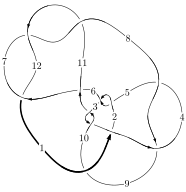
\includegraphics[width=112pt]{../../../GIT/diagram.site/Diagrams/png/2884_12n_0795.png}\\
\ \ \ A knot diagram\footnotemark}&
\allowdisplaybreaks
\textbf{Linearized knot diagam} \\
\cline{2-2}
 &
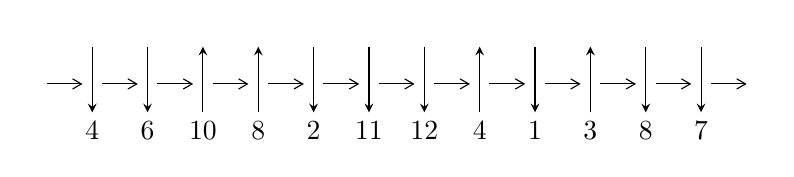
\begin{tikzpicture}[x=20pt, y=17pt]
	% nodes
	\node (C0) at (0, 0) {};
	\node (C1) at (1, 0) {};
	\node (C1U) at (1, +1) {};
	\node (C1D) at (1, -1) {4};

	\node (C2) at (2, 0) {};
	\node (C2U) at (2, +1) {};
	\node (C2D) at (2, -1) {6};

	\node (C3) at (3, 0) {};
	\node (C3U) at (3, +1) {};
	\node (C3D) at (3, -1) {10};

	\node (C4) at (4, 0) {};
	\node (C4U) at (4, +1) {};
	\node (C4D) at (4, -1) {8};

	\node (C5) at (5, 0) {};
	\node (C5U) at (5, +1) {};
	\node (C5D) at (5, -1) {2};

	\node (C6) at (6, 0) {};
	\node (C6U) at (6, +1) {};
	\node (C6D) at (6, -1) {11};

	\node (C7) at (7, 0) {};
	\node (C7U) at (7, +1) {};
	\node (C7D) at (7, -1) {12};

	\node (C8) at (8, 0) {};
	\node (C8U) at (8, +1) {};
	\node (C8D) at (8, -1) {4};

	\node (C9) at (9, 0) {};
	\node (C9U) at (9, +1) {};
	\node (C9D) at (9, -1) {1};

	\node (C10) at (10, 0) {};
	\node (C10U) at (10, +1) {};
	\node (C10D) at (10, -1) {3};

	\node (C11) at (11, 0) {};
	\node (C11U) at (11, +1) {};
	\node (C11D) at (11, -1) {8};

	\node (C12) at (12, 0) {};
	\node (C12U) at (12, +1) {};
	\node (C12D) at (12, -1) {7};
	\node (C13) at (13, 0) {};

	% arrows
	\draw[->,>={angle 60}]
	(C0) edge (C1) (C1) edge (C2) (C2) edge (C3) (C3) edge (C4) (C4) edge (C5) (C5) edge (C6) (C6) edge (C7) (C7) edge (C8) (C8) edge (C9) (C9) edge (C10) (C10) edge (C11) (C11) edge (C12) (C12) edge (C13) ;	\draw[->,>=stealth]
	(C1U) edge (C1D) (C2U) edge (C2D) (C3D) edge (C3U) (C4D) edge (C4U) (C5U) edge (C5D) (C6U) edge (C6D) (C7U) edge (C7D) (C8D) edge (C8U) (C9U) edge (C9D) (C10D) edge (C10U) (C11U) edge (C11D) (C12U) edge (C12D) ;
	\end{tikzpicture} \\
\hhline{~~} \\& 
\textbf{Solving Sequence} \\ \cline{2-2} 
 &
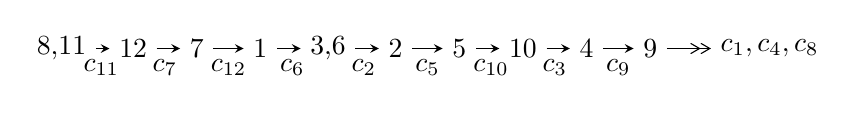
\begin{tikzpicture}[x=23pt, y=7pt]
	% node
	\node (A0) at (-1/8, 0) {8,11};
	\node (A1) at (1, 0) {12};
	\node (A2) at (2, 0) {7};
	\node (A3) at (3, 0) {1};
	\node (A4) at (65/16, 0) {3,6};
	\node (A5) at (41/8, 0) {2};
	\node (A6) at (49/8, 0) {5};
	\node (A7) at (57/8, 0) {10};
	\node (A8) at (65/8, 0) {4};
	\node (A9) at (73/8, 0) {9};
	\node (C1) at (1/2, -1) {$c_{11}$};
	\node (C2) at (3/2, -1) {$c_{7}$};
	\node (C3) at (5/2, -1) {$c_{12}$};
	\node (C4) at (7/2, -1) {$c_{6}$};
	\node (C5) at (37/8, -1) {$c_{2}$};
	\node (C6) at (45/8, -1) {$c_{5}$};
	\node (C7) at (53/8, -1) {$c_{10}$};
	\node (C8) at (61/8, -1) {$c_{3}$};
	\node (C9) at (69/8, -1) {$c_{9}$};
	\node (A10) at (11, 0) {$c_{1},c_{4},c_{8}$};

	% edge
	\draw[->,>=stealth]	
	(A0) edge (A1) (A1) edge (A2) (A2) edge (A3) (A3) edge (A4) (A4) edge (A5) (A5) edge (A6) (A6) edge (A7) (A7) edge (A8) (A8) edge (A9) ;
	\draw[->>,>={angle 60}]	
	(A9) edge (A10);
\end{tikzpicture} \\ 

\end{tabular} \\

\footnotetext{
The image of knot diagram is generated by the software ``\textbf{Draw programme}" developed by Andrew Bartholomew(\url{http://www.layer8.co.uk/maths/draw/index.htm\#Running-draw}), where we modified some parts for our purpose(\url{https://github.com/CATsTAILs/LinksPainter}).
}\phantom \\ \newline 
\centering \textbf{Ideals for irreducible components\footnotemark of $X_{\text{par}}$} 
 
\begin{align*}
I^u_{1}&=\langle 
-1.02240\times10^{36} u^{53}-1.89768\times10^{37} u^{52}+\cdots+3.08931\times10^{37} b+8.64765\times10^{37},\\
\phantom{I^u_{1}}&\phantom{= \langle  }-3.79905\times10^{37} u^{53}-2.32864\times10^{37} u^{52}+\cdots+3.39824\times10^{38} a+7.15973\times10^{38},\\
\phantom{I^u_{1}}&\phantom{= \langle  }u^{54}+2 u^{53}+\cdots-68 u-11\rangle \\
I^u_{2}&=\langle 
- u^{14}-7 u^{12}-18 u^{10}+u^9-19 u^8+5 u^7-4 u^6+7 u^5+3 u^4+u^3- u^2+b-3 u,\\
\phantom{I^u_{2}}&\phantom{= \langle  }- u^{14}+2 u^{13}-9 u^{12}+15 u^{11}-31 u^{10}+43 u^9-50 u^8+56 u^7-35 u^6+26 u^5-3 u^4-6 u^3+7 u^2+a-5 u+4,\\
\phantom{I^u_{2}}&\phantom{= \langle  }u^{15}- u^{14}+9 u^{13}-8 u^{12}+32 u^{11}-25 u^{10}+55 u^9-37 u^8+42 u^7-22 u^6+4 u^5+3 u^4-8 u^3+7 u^2+1\rangle \\
\\
\end{align*}
\raggedright * 2 irreducible components of $\dim_{\mathbb{C}}=0$, with total 69 representations.\\
\footnotetext{All coefficients of polynomials are rational numbers. But the coefficients are sometimes approximated in decimal forms when there is not enough margin.}
\newpage
\renewcommand{\arraystretch}{1}
\centering \section*{I. $I^u_{1}= \langle -1.02\times10^{36} u^{53}-1.90\times10^{37} u^{52}+\cdots+3.09\times10^{37} b+8.65\times10^{37},\;-3.80\times10^{37} u^{53}-2.33\times10^{37} u^{52}+\cdots+3.40\times10^{38} a+7.16\times10^{38},\;u^{54}+2 u^{53}+\cdots-68 u-11 \rangle$}
\flushleft \textbf{(i) Arc colorings}\\
\begin{tabular}{m{7pt} m{180pt} m{7pt} m{180pt} }
\flushright $a_{8}=$&$\begin{pmatrix}0\\u\end{pmatrix}$ \\
\flushright $a_{11}=$&$\begin{pmatrix}1\\0\end{pmatrix}$ \\
\flushright $a_{12}=$&$\begin{pmatrix}1\\u^2\end{pmatrix}$ \\
\flushright $a_{7}=$&$\begin{pmatrix}u\\u^3+u\end{pmatrix}$ \\
\flushright $a_{1}=$&$\begin{pmatrix}u^2+1\\u^4+2 u^2\end{pmatrix}$ \\
\flushright $a_{3}=$&$\begin{pmatrix}0.111794 u^{53}+0.0685248 u^{52}+\cdots-6.32751 u-2.10689\\0.0330947 u^{53}+0.614273 u^{52}+\cdots-14.1115 u-2.79922\end{pmatrix}$ \\
\flushright $a_{6}=$&$\begin{pmatrix}u^3+2 u\\u^3+u\end{pmatrix}$ \\
\flushright $a_{2}=$&$\begin{pmatrix}-0.0462518 u^{53}-0.197231 u^{52}+\cdots+18.3660 u+3.41252\\-0.0768640 u^{53}+0.598332 u^{52}+\cdots-7.25300 u-0.884533\end{pmatrix}$ \\
\flushright $a_{5}=$&$\begin{pmatrix}0.598411 u^{53}+0.724886 u^{52}+\cdots-4.83758 u-2.53344\\0.644293 u^{53}+0.0999628 u^{52}+\cdots+2.37484 u-0.981251\end{pmatrix}$ \\
\flushright $a_{10}=$&$\begin{pmatrix}0.869370 u^{53}+1.10346 u^{52}+\cdots-57.0809 u-12.2337\\0.758825 u^{53}+2.10666 u^{52}+\cdots-76.2371 u-14.3877\end{pmatrix}$ \\
\flushright $a_{4}=$&$\begin{pmatrix}-0.598411 u^{53}-0.724886 u^{52}+\cdots+4.83758 u+2.53344\\0.0503708 u^{53}+0.206592 u^{52}+\cdots+23.1342 u+6.17254\end{pmatrix}$ \\
\flushright $a_{9}=$&$\begin{pmatrix}1.21296 u^{53}+1.80879 u^{52}+\cdots-76.8483 u-15.7970\\0.882160 u^{53}+2.58325 u^{52}+\cdots-91.2590 u-17.2428\end{pmatrix}$\\&\end{tabular}
\flushleft \textbf{(ii) Obstruction class $= -1$}\\~\\
\flushleft \textbf{(iii) Cusp Shapes $= -0.660515 u^{53}-1.00096 u^{52}+\cdots-64.0934 u-26.6095$}\\~\\
\newpage\renewcommand{\arraystretch}{1}
\flushleft \textbf{(iv) u-Polynomials at the component}\newline \\
\begin{tabular}{m{50pt}|m{274pt}}
Crossings & \hspace{64pt}u-Polynomials at each crossing \\
\hline $$\begin{aligned}c_{1}\end{aligned}$$&$\begin{aligned}
&u^{54}- u^{53}+\cdots+161 u-7
\end{aligned}$\\
\hline $$\begin{aligned}c_{2},c_{5}\end{aligned}$$&$\begin{aligned}
&u^{54}+4 u^{53}+\cdots+100 u-7
\end{aligned}$\\
\hline $$\begin{aligned}c_{3},c_{10}\end{aligned}$$&$\begin{aligned}
&u^{54}+u^{53}+\cdots-24 u+79
\end{aligned}$\\
\hline $$\begin{aligned}c_{4},c_{8}\end{aligned}$$&$\begin{aligned}
&u^{54}-3 u^{53}+\cdots-1056 u+279
\end{aligned}$\\
\hline $$\begin{aligned}c_{6}\end{aligned}$$&$\begin{aligned}
&u^{54}-2 u^{53}+\cdots-9058 u-3839
\end{aligned}$\\
\hline $$\begin{aligned}c_{7},c_{11},c_{12}\end{aligned}$$&$\begin{aligned}
&u^{54}+2 u^{53}+\cdots-68 u-11
\end{aligned}$\\
\hline $$\begin{aligned}c_{9}\end{aligned}$$&$\begin{aligned}
&u^{54}+u^{53}+\cdots+34 u-1
\end{aligned}$\\
\hline
\end{tabular}\\~\\
\newpage\renewcommand{\arraystretch}{1}
\flushleft \textbf{(v) Riley Polynomials at the component}\newline \\
\begin{tabular}{m{50pt}|m{274pt}}
Crossings & \hspace{64pt}Riley Polynomials at each crossing \\
\hline $$\begin{aligned}c_{1}\end{aligned}$$&$\begin{aligned}
&y^{54}+53 y^{53}+\cdots-8141 y+49
\end{aligned}$\\
\hline $$\begin{aligned}c_{2},c_{5}\end{aligned}$$&$\begin{aligned}
&y^{54}-22 y^{53}+\cdots-10854 y+49
\end{aligned}$\\
\hline $$\begin{aligned}c_{3},c_{10}\end{aligned}$$&$\begin{aligned}
&y^{54}+49 y^{53}+\cdots-26804 y+6241
\end{aligned}$\\
\hline $$\begin{aligned}c_{4},c_{8}\end{aligned}$$&$\begin{aligned}
&y^{54}-59 y^{53}+\cdots-3109428 y+77841
\end{aligned}$\\
\hline $$\begin{aligned}c_{6}\end{aligned}$$&$\begin{aligned}
&y^{54}+4 y^{53}+\cdots+184125862 y+14737921
\end{aligned}$\\
\hline $$\begin{aligned}c_{7},c_{11},c_{12}\end{aligned}$$&$\begin{aligned}
&y^{54}+52 y^{53}+\cdots-1082 y+121
\end{aligned}$\\
\hline $$\begin{aligned}c_{9}\end{aligned}$$&$\begin{aligned}
&y^{54}+55 y^{53}+\cdots-1762 y+1
\end{aligned}$\\
\hline
\end{tabular}\\~\\
\newpage\flushleft \textbf{(vi) Complex Volumes and Cusp Shapes}
$$\begin{array}{c|c|c}  
\text{Solutions to }I^u_{1}& \I (\text{vol} + \sqrt{-1}CS) & \text{Cusp shape}\\
 \hline 
\begin{aligned}
u &= -0.881137 + 0.332755 I \\
a &= \phantom{-}0.54399 - 2.13485 I \\
b &= -0.39987 - 1.44588 I\end{aligned}
 & -1.46224 + 9.75579 I & -6.92865 - 6.33368 I \\ \hline\begin{aligned}
u &= -0.881137 - 0.332755 I \\
a &= \phantom{-}0.54399 + 2.13485 I \\
b &= -0.39987 + 1.44588 I\end{aligned}
 & -1.46224 - 9.75579 I & -6.92865 + 6.33368 I \\ \hline\begin{aligned}
u &= -0.661598 + 0.849697 I \\
a &= \phantom{-}0.701547 - 1.110120 I \\
b &= \phantom{-}0.308972 - 1.370990 I\end{aligned}
 & \phantom{-}0.12696 - 4.49631 I & -5.88481 + 2.41612 I \\ \hline\begin{aligned}
u &= -0.661598 - 0.849697 I \\
a &= \phantom{-}0.701547 + 1.110120 I \\
b &= \phantom{-}0.308972 + 1.370990 I\end{aligned}
 & \phantom{-}0.12696 + 4.49631 I & -5.88481 - 2.41612 I \\ \hline\begin{aligned}
u &= \phantom{-}0.862493 + 0.086515 I \\
a &= -0.43056 - 2.27902 I \\
b &= \phantom{-}0.194758 - 1.252480 I\end{aligned}
 & -5.81257 - 2.56927 I & -8.23844 + 3.31387 I \\ \hline\begin{aligned}
u &= \phantom{-}0.862493 - 0.086515 I \\
a &= -0.43056 + 2.27902 I \\
b &= \phantom{-}0.194758 + 1.252480 I\end{aligned}
 & -5.81257 + 2.56927 I & -8.23844 - 3.31387 I \\ \hline\begin{aligned}
u &= \phantom{-}0.034093 + 1.169890 I \\
a &= \phantom{-}0.694656 + 1.176320 I \\
b &= -0.07515 + 1.63362 I\end{aligned}
 & -5.56210 - 0.29699 I & \phantom{-0.000000 } 0 \\ \hline\begin{aligned}
u &= \phantom{-}0.034093 - 1.169890 I \\
a &= \phantom{-}0.694656 - 1.176320 I \\
b &= -0.07515 - 1.63362 I\end{aligned}
 & -5.56210 + 0.29699 I & \phantom{-0.000000 } 0 \\ \hline\begin{aligned}
u &= -0.061275 + 1.202860 I \\
a &= -1.171810 - 0.220502 I \\
b &= \phantom{-}0.682474 + 0.808517 I\end{aligned}
 & \phantom{-}4.62735 + 2.61524 I & \phantom{-0.000000 } 0 \\ \hline\begin{aligned}
u &= -0.061275 - 1.202860 I \\
a &= -1.171810 + 0.220502 I \\
b &= \phantom{-}0.682474 - 0.808517 I\end{aligned}
 & \phantom{-}4.62735 - 2.61524 I & \phantom{-0.000000 } 0\\
 \hline 
 \end{array}$$\newpage$$\begin{array}{c|c|c}  
\text{Solutions to }I^u_{1}& \I (\text{vol} + \sqrt{-1}CS) & \text{Cusp shape}\\
 \hline 
\begin{aligned}
u &= \phantom{-}0.703654 + 0.331302 I \\
a &= -0.449981 + 0.493740 I \\
b &= -0.953667 + 0.272713 I\end{aligned}
 & \phantom{-}3.98978 - 4.89959 I & -3.74361 + 5.61016 I \\ \hline\begin{aligned}
u &= \phantom{-}0.703654 - 0.331302 I \\
a &= -0.449981 - 0.493740 I \\
b &= -0.953667 - 0.272713 I\end{aligned}
 & \phantom{-}3.98978 + 4.89959 I & -3.74361 - 5.61016 I \\ \hline\begin{aligned}
u &= \phantom{-}0.517589 + 0.579128 I \\
a &= \phantom{-}0.432842 - 1.079910 I \\
b &= \phantom{-}0.686610 + 0.121861 I\end{aligned}
 & \phantom{-}4.91286 + 0.83348 I & -0.991616 + 0.466967 I \\ \hline\begin{aligned}
u &= \phantom{-}0.517589 - 0.579128 I \\
a &= \phantom{-}0.432842 + 1.079910 I \\
b &= \phantom{-}0.686610 - 0.121861 I\end{aligned}
 & \phantom{-}4.91286 - 0.83348 I & -0.991616 - 0.466967 I \\ \hline\begin{aligned}
u &= -0.660016 + 0.406956 I \\
a &= -1.06148 + 1.12929 I \\
b &= \phantom{-}0.127395 + 1.287570 I\end{aligned}
 & -6.55286 + 2.04235 I & -7.25331 - 3.50673 I \\ \hline\begin{aligned}
u &= -0.660016 - 0.406956 I \\
a &= -1.06148 - 1.12929 I \\
b &= \phantom{-}0.127395 - 1.287570 I\end{aligned}
 & -6.55286 - 2.04235 I & -7.25331 + 3.50673 I \\ \hline\begin{aligned}
u &= -0.152086 + 1.230400 I \\
a &= -2.21560 + 0.95171 I \\
b &= -0.022858 + 1.045750 I\end{aligned}
 & \phantom{-}4.59893 - 0.06572 I & \phantom{-0.000000 } 0 \\ \hline\begin{aligned}
u &= -0.152086 - 1.230400 I \\
a &= -2.21560 - 0.95171 I \\
b &= -0.022858 - 1.045750 I\end{aligned}
 & \phantom{-}4.59893 + 0.06572 I & \phantom{-0.000000 } 0 \\ \hline\begin{aligned}
u &= \phantom{-}0.464769 + 1.178440 I \\
a &= -0.444192 - 1.161940 I \\
b &= -0.045829 - 1.278020 I\end{aligned}
 & -2.46094 - 2.14351 I & \phantom{-0.000000 } 0 \\ \hline\begin{aligned}
u &= \phantom{-}0.464769 - 1.178440 I \\
a &= -0.444192 + 1.161940 I \\
b &= -0.045829 + 1.278020 I\end{aligned}
 & -2.46094 + 2.14351 I & \phantom{-0.000000 } 0\\
 \hline 
 \end{array}$$\newpage$$\begin{array}{c|c|c}  
\text{Solutions to }I^u_{1}& \I (\text{vol} + \sqrt{-1}CS) & \text{Cusp shape}\\
 \hline 
\begin{aligned}
u &= -0.718867\phantom{ +0.000000I} \\
a &= \phantom{-}0.234022\phantom{ +0.000000I} \\
b &= \phantom{-}0.516900\phantom{ +0.000000I}\end{aligned}
 & -2.00172\phantom{ +0.000000I} & -2.11670\phantom{ +0.000000I} \\ \hline\begin{aligned}
u &= \phantom{-}0.618358 + 0.333206 I \\
a &= \phantom{-}1.21587 + 2.22737 I \\
b &= -0.07061 + 1.56445 I\end{aligned}
 & -7.42325 - 1.74416 I & -4.39978 + 3.82440 I \\ \hline\begin{aligned}
u &= \phantom{-}0.618358 - 0.333206 I \\
a &= \phantom{-}1.21587 - 2.22737 I \\
b &= -0.07061 - 1.56445 I\end{aligned}
 & -7.42325 + 1.74416 I & -4.39978 - 3.82440 I \\ \hline\begin{aligned}
u &= -0.300837 + 1.283390 I \\
a &= \phantom{-}0.334898 - 0.433885 I \\
b &= -0.533318 + 0.132363 I\end{aligned}
 & \phantom{-}2.00821 + 3.67955 I & \phantom{-0.000000 } 0 \\ \hline\begin{aligned}
u &= -0.300837 - 1.283390 I \\
a &= \phantom{-}0.334898 + 0.433885 I \\
b &= -0.533318 - 0.132363 I\end{aligned}
 & \phantom{-}2.00821 - 3.67955 I & \phantom{-0.000000 } 0 \\ \hline\begin{aligned}
u &= \phantom{-}0.154982 + 1.323550 I \\
a &= \phantom{-}0.726837 - 0.314235 I \\
b &= -0.614893 - 0.397811 I\end{aligned}
 & \phantom{-}1.72966 - 2.23286 I & \phantom{-0.000000 } 0 \\ \hline\begin{aligned}
u &= \phantom{-}0.154982 - 1.323550 I \\
a &= \phantom{-}0.726837 + 0.314235 I \\
b &= -0.614893 + 0.397811 I\end{aligned}
 & \phantom{-}1.72966 + 2.23286 I & \phantom{-0.000000 } 0 \\ \hline\begin{aligned}
u &= -0.094235 + 1.347490 I \\
a &= -0.883756 + 0.145148 I \\
b &= \phantom{-}0.620923 + 0.478168 I\end{aligned}
 & \phantom{-}4.77656 + 2.05407 I & \phantom{-0.000000 } 0 \\ \hline\begin{aligned}
u &= -0.094235 - 1.347490 I \\
a &= -0.883756 - 0.145148 I \\
b &= \phantom{-}0.620923 - 0.478168 I\end{aligned}
 & \phantom{-}4.77656 - 2.05407 I & \phantom{-0.000000 } 0 \\ \hline\begin{aligned}
u &= \phantom{-}0.376292 + 1.326680 I \\
a &= \phantom{-}1.34754 + 1.24800 I \\
b &= -0.310469 + 1.232490 I\end{aligned}
 & -1.38617 - 7.00293 I & \phantom{-0.000000 } 0\\
 \hline 
 \end{array}$$\newpage$$\begin{array}{c|c|c}  
\text{Solutions to }I^u_{1}& \I (\text{vol} + \sqrt{-1}CS) & \text{Cusp shape}\\
 \hline 
\begin{aligned}
u &= \phantom{-}0.376292 - 1.326680 I \\
a &= \phantom{-}1.34754 - 1.24800 I \\
b &= -0.310469 - 1.232490 I\end{aligned}
 & -1.38617 + 7.00293 I & \phantom{-0.000000 } 0 \\ \hline\begin{aligned}
u &= -0.229873 + 1.369020 I \\
a &= \phantom{-}1.07939 - 1.70290 I \\
b &= -0.34520 - 1.44114 I\end{aligned}
 & \phantom{-}6.29624 + 5.50512 I & \phantom{-0.000000 } 0 \\ \hline\begin{aligned}
u &= -0.229873 - 1.369020 I \\
a &= \phantom{-}1.07939 + 1.70290 I \\
b &= -0.34520 + 1.44114 I\end{aligned}
 & \phantom{-}6.29624 - 5.50512 I & \phantom{-0.000000 } 0 \\ \hline\begin{aligned}
u &= -0.201736 + 1.374670 I \\
a &= -0.069667 - 0.195301 I \\
b &= \phantom{-}0.77398 - 1.23082 I\end{aligned}
 & \phantom{-}6.68190 + 1.90913 I & \phantom{-0.000000 } 0 \\ \hline\begin{aligned}
u &= -0.201736 - 1.374670 I \\
a &= -0.069667 + 0.195301 I \\
b &= \phantom{-}0.77398 + 1.23082 I\end{aligned}
 & \phantom{-}6.68190 - 1.90913 I & \phantom{-0.000000 } 0 \\ \hline\begin{aligned}
u &= -0.569109 + 0.157556 I \\
a &= \phantom{-}0.21924 + 4.04070 I \\
b &= \phantom{-}0.271278 + 1.251950 I\end{aligned}
 & \phantom{-}1.40834 + 2.55636 I & -7.88899 - 3.76167 I \\ \hline\begin{aligned}
u &= -0.569109 - 0.157556 I \\
a &= \phantom{-}0.21924 - 4.04070 I \\
b &= \phantom{-}0.271278 - 1.251950 I\end{aligned}
 & \phantom{-}1.40834 - 2.55636 I & -7.88899 + 3.76167 I \\ \hline\begin{aligned}
u &= \phantom{-}0.26439 + 1.43158 I \\
a &= -1.176170 - 0.713113 I \\
b &= \phantom{-}0.20131 - 1.51219 I\end{aligned}
 & -1.76307 - 5.05086 I & \phantom{-0.000000 } 0 \\ \hline\begin{aligned}
u &= \phantom{-}0.26439 - 1.43158 I \\
a &= -1.176170 + 0.713113 I \\
b &= \phantom{-}0.20131 + 1.51219 I\end{aligned}
 & -1.76307 + 5.05086 I & \phantom{-0.000000 } 0 \\ \hline\begin{aligned}
u &= \phantom{-}0.27745 + 1.43289 I \\
a &= -0.482110 - 0.560176 I \\
b &= \phantom{-}1.128380 - 0.228809 I\end{aligned}
 & \phantom{-}9.62901 - 8.48480 I & \phantom{-0.000000 } 0\\
 \hline 
 \end{array}$$\newpage$$\begin{array}{c|c|c}  
\text{Solutions to }I^u_{1}& \I (\text{vol} + \sqrt{-1}CS) & \text{Cusp shape}\\
 \hline 
\begin{aligned}
u &= \phantom{-}0.27745 - 1.43289 I \\
a &= -0.482110 + 0.560176 I \\
b &= \phantom{-}1.128380 + 0.228809 I\end{aligned}
 & \phantom{-}9.62901 + 8.48480 I & \phantom{-0.000000 } 0 \\ \hline\begin{aligned}
u &= -0.501917 + 0.181939 I \\
a &= -0.02666 + 1.76555 I \\
b &= -0.658368 + 1.057790 I\end{aligned}
 & \phantom{-}1.69160 - 0.71190 I & -8.63375 - 2.05858 I \\ \hline\begin{aligned}
u &= -0.501917 - 0.181939 I \\
a &= -0.02666 - 1.76555 I \\
b &= -0.658368 - 1.057790 I\end{aligned}
 & \phantom{-}1.69160 + 0.71190 I & -8.63375 + 2.05858 I \\ \hline\begin{aligned}
u &= -0.27382 + 1.46493 I \\
a &= \phantom{-}1.043680 - 0.263678 I \\
b &= -0.267903 - 1.143590 I\end{aligned}
 & -0.53926 + 5.52355 I & \phantom{-0.000000 } 0 \\ \hline\begin{aligned}
u &= -0.27382 - 1.46493 I \\
a &= \phantom{-}1.043680 + 0.263678 I \\
b &= -0.267903 + 1.143590 I\end{aligned}
 & -0.53926 - 5.52355 I & \phantom{-0.000000 } 0 \\ \hline\begin{aligned}
u &= -0.35422 + 1.45911 I \\
a &= -1.24409 + 1.06931 I \\
b &= \phantom{-}0.48568 + 1.47325 I\end{aligned}
 & \phantom{-}4.2552 + 14.2219 I & \phantom{-0.000000 } 0 \\ \hline\begin{aligned}
u &= -0.35422 - 1.45911 I \\
a &= -1.24409 - 1.06931 I \\
b &= \phantom{-}0.48568 - 1.47325 I\end{aligned}
 & \phantom{-}4.2552 - 14.2219 I & \phantom{-0.000000 } 0 \\ \hline\begin{aligned}
u &= \phantom{-}0.14172 + 1.50342 I \\
a &= \phantom{-}0.239640 + 0.749072 I \\
b &= -0.722793 + 0.242786 I\end{aligned}
 & \phantom{-}11.72290 - 1.51265 I & \phantom{-0.000000 } 0 \\ \hline\begin{aligned}
u &= \phantom{-}0.14172 - 1.50342 I \\
a &= \phantom{-}0.239640 - 0.749072 I \\
b &= -0.722793 - 0.242786 I\end{aligned}
 & \phantom{-}11.72290 + 1.51265 I & \phantom{-0.000000 } 0 \\ \hline\begin{aligned}
u &= \phantom{-}0.475960\phantom{ +0.000000I} \\
a &= -1.20947\phantom{ +0.000000I} \\
b &= \phantom{-}0.452125\phantom{ +0.000000I}\end{aligned}
 & -2.46570\phantom{ +0.000000I} & \phantom{-}2.76380\phantom{ +0.000000I}\\
 \hline 
 \end{array}$$\newpage$$\begin{array}{c|c|c}  
\text{Solutions to }I^u_{1}& \I (\text{vol} + \sqrt{-1}CS) & \text{Cusp shape}\\
 \hline 
\begin{aligned}
u &= -0.254809 + 0.273319 I \\
a &= \phantom{-}0.778345 - 0.766727 I \\
b &= -0.196995 - 0.477015 I\end{aligned}
 & -0.216037 + 0.828510 I & -5.24914 - 8.37217 I \\ \hline\begin{aligned}
u &= -0.254809 - 0.273319 I \\
a &= \phantom{-}0.778345 + 0.766727 I \\
b &= -0.196995 + 0.477015 I\end{aligned}
 & -0.216037 - 0.828510 I & -5.24914 + 8.37217 I \\ \hline\begin{aligned}
u &= -0.09766 + 1.65580 I \\
a &= -0.169231 + 0.249301 I \\
b &= -0.248336 + 1.196290 I\end{aligned}
 & \phantom{-}8.90251 - 1.85529 I & \phantom{-0.000000 } 0 \\ \hline\begin{aligned}
u &= -0.09766 - 1.65580 I \\
a &= -0.169231 - 0.249301 I \\
b &= -0.248336 - 1.196290 I\end{aligned}
 & \phantom{-}8.90251 + 1.85529 I & \phantom{-0.000000 } 0\\
 \hline 
 \end{array}$$\newpage\newpage\renewcommand{\arraystretch}{1}
\centering \section*{II. $I^u_{2}= \langle - u^{14}-7 u^{12}+\cdots+b-3 u,\;- u^{14}+2 u^{13}+\cdots+a+4,\;u^{15}- u^{14}+\cdots+7 u^2+1 \rangle$}
\flushleft \textbf{(i) Arc colorings}\\
\begin{tabular}{m{7pt} m{180pt} m{7pt} m{180pt} }
\flushright $a_{8}=$&$\begin{pmatrix}0\\u\end{pmatrix}$ \\
\flushright $a_{11}=$&$\begin{pmatrix}1\\0\end{pmatrix}$ \\
\flushright $a_{12}=$&$\begin{pmatrix}1\\u^2\end{pmatrix}$ \\
\flushright $a_{7}=$&$\begin{pmatrix}u\\u^3+u\end{pmatrix}$ \\
\flushright $a_{1}=$&$\begin{pmatrix}u^2+1\\u^4+2 u^2\end{pmatrix}$ \\
\flushright $a_{3}=$&$\begin{pmatrix}u^{14}-2 u^{13}+\cdots+5 u-4\\u^{14}+7 u^{12}+18 u^{10}- u^9+19 u^8-5 u^7+4 u^6-7 u^5-3 u^4- u^3+u^2+3 u\end{pmatrix}$ \\
\flushright $a_{6}=$&$\begin{pmatrix}u^3+2 u\\u^3+u\end{pmatrix}$ \\
\flushright $a_{2}=$&$\begin{pmatrix}- u^{13}+u^{12}+\cdots+4 u-4\\u^{14}+7 u^{12}+18 u^{10}- u^9+19 u^8-5 u^7+4 u^6-7 u^5-2 u^4- u^3+3 u^2+3 u\end{pmatrix}$ \\
\flushright $a_{5}=$&$\begin{pmatrix}u^{14}-2 u^{13}+\cdots+10 u-1\\-2 u^{13}+2 u^{12}+\cdots+2 u-1\end{pmatrix}$ \\
\flushright $a_{10}=$&$\begin{pmatrix}-2 u^{14}+2 u^{13}+\cdots-11 u+1\\u^{13}- u^{12}+\cdots+6 u^2-2 u\end{pmatrix}$ \\
\flushright $a_{4}=$&$\begin{pmatrix}u^{14}-2 u^{13}+\cdots+10 u-1\\- u^{13}+u^{12}+\cdots-5 u^2+u\end{pmatrix}$ \\
\flushright $a_{9}=$&$\begin{pmatrix}-2 u^{14}+2 u^{13}+\cdots-14 u+1\\u^{13}- u^{12}+\cdots+6 u^2- u\end{pmatrix}$\\&\end{tabular}
\flushleft \textbf{(ii) Obstruction class $= 1$}\\~\\
\flushleft \textbf{(iii) Cusp Shapes $= -3 u^{14}+6 u^{13}-24 u^{12}+42 u^{11}-71 u^{10}+108 u^9-89 u^8+115 u^7-33 u^6+25 u^5+9 u^4-22 u^3-4 u^2+2 u-3$}\\~\\
\newpage\renewcommand{\arraystretch}{1}
\flushleft \textbf{(iv) u-Polynomials at the component}\newline \\
\begin{tabular}{m{50pt}|m{274pt}}
Crossings & \hspace{64pt}u-Polynomials at each crossing \\
\hline $$\begin{aligned}c_{1}\end{aligned}$$&$\begin{aligned}
&u^{15}+3 u^{13}+\cdots-3 u-1
\end{aligned}$\\
\hline $$\begin{aligned}c_{2}\end{aligned}$$&$\begin{aligned}
&u^{15}+3 u^{14}+\cdots-3 u^2-1
\end{aligned}$\\
\hline $$\begin{aligned}c_{3}\end{aligned}$$&$\begin{aligned}
&u^{15}+9 u^{13}+\cdots-4 u^2+1
\end{aligned}$\\
\hline $$\begin{aligned}c_{4}\end{aligned}$$&$\begin{aligned}
&u^{15}-2 u^{14}+\cdots+10 u^2-1
\end{aligned}$\\
\hline $$\begin{aligned}c_{5}\end{aligned}$$&$\begin{aligned}
&u^{15}-3 u^{14}+\cdots+3 u^2+1
\end{aligned}$\\
\hline $$\begin{aligned}c_{6}\end{aligned}$$&$\begin{aligned}
&u^{15}- u^{14}+\cdots+2 u-1
\end{aligned}$\\
\hline $$\begin{aligned}c_{7}\end{aligned}$$&$\begin{aligned}
&u^{15}+u^{14}+\cdots-7 u^2-1
\end{aligned}$\\
\hline $$\begin{aligned}c_{8}\end{aligned}$$&$\begin{aligned}
&u^{15}+2 u^{14}+\cdots-10 u^2+1
\end{aligned}$\\
\hline $$\begin{aligned}c_{9}\end{aligned}$$&$\begin{aligned}
&u^{15}+6 u^{13}+\cdots+3 u^2-1
\end{aligned}$\\
\hline $$\begin{aligned}c_{10}\end{aligned}$$&$\begin{aligned}
&u^{15}+9 u^{13}+\cdots+4 u^2-1
\end{aligned}$\\
\hline $$\begin{aligned}c_{11},c_{12}\end{aligned}$$&$\begin{aligned}
&u^{15}- u^{14}+\cdots+7 u^2+1
\end{aligned}$\\
\hline
\end{tabular}\\~\\
\newpage\renewcommand{\arraystretch}{1}
\flushleft \textbf{(v) Riley Polynomials at the component}\newline \\
\begin{tabular}{m{50pt}|m{274pt}}
Crossings & \hspace{64pt}Riley Polynomials at each crossing \\
\hline $$\begin{aligned}c_{1}\end{aligned}$$&$\begin{aligned}
&y^{15}+6 y^{14}+\cdots+9 y-1
\end{aligned}$\\
\hline $$\begin{aligned}c_{2},c_{5}\end{aligned}$$&$\begin{aligned}
&y^{15}-9 y^{14}+\cdots-6 y-1
\end{aligned}$\\
\hline $$\begin{aligned}c_{3},c_{10}\end{aligned}$$&$\begin{aligned}
&y^{15}+18 y^{14}+\cdots+8 y-1
\end{aligned}$\\
\hline $$\begin{aligned}c_{4},c_{8}\end{aligned}$$&$\begin{aligned}
&y^{15}-6 y^{14}+\cdots+20 y-1
\end{aligned}$\\
\hline $$\begin{aligned}c_{6}\end{aligned}$$&$\begin{aligned}
&y^{15}+5 y^{14}+\cdots-18 y-1
\end{aligned}$\\
\hline $$\begin{aligned}c_{7},c_{11},c_{12}\end{aligned}$$&$\begin{aligned}
&y^{15}+17 y^{14}+\cdots-14 y-1
\end{aligned}$\\
\hline $$\begin{aligned}c_{9}\end{aligned}$$&$\begin{aligned}
&y^{15}+12 y^{14}+\cdots+6 y-1
\end{aligned}$\\
\hline
\end{tabular}\\~\\
\newpage\flushleft \textbf{(vi) Complex Volumes and Cusp Shapes}
$$\begin{array}{c|c|c}  
\text{Solutions to }I^u_{2}& \I (\text{vol} + \sqrt{-1}CS) & \text{Cusp shape}\\
 \hline 
\begin{aligned}
u &= \phantom{-}0.203897 + 1.182510 I \\
a &= -0.354319 - 1.221590 I \\
b &= -0.08173 - 1.61035 I\end{aligned}
 & -5.71687 - 1.52845 I & -6.08651 + 4.82612 I \\ \hline\begin{aligned}
u &= \phantom{-}0.203897 - 1.182510 I \\
a &= -0.354319 + 1.221590 I \\
b &= -0.08173 + 1.61035 I\end{aligned}
 & -5.71687 + 1.52845 I & -6.08651 - 4.82612 I \\ \hline\begin{aligned}
u &= -0.033799 + 1.247150 I \\
a &= -1.91300 + 0.07166 I \\
b &= \phantom{-}0.496329 + 0.968310 I\end{aligned}
 & \phantom{-}5.47176 + 1.87806 I & \phantom{-}1.95765 - 1.95299 I \\ \hline\begin{aligned}
u &= -0.033799 - 1.247150 I \\
a &= -1.91300 - 0.07166 I \\
b &= \phantom{-}0.496329 - 0.968310 I\end{aligned}
 & \phantom{-}5.47176 - 1.87806 I & \phantom{-}1.95765 + 1.95299 I \\ \hline\begin{aligned}
u &= \phantom{-}0.695741 + 0.257174 I \\
a &= -1.14939 - 2.10113 I \\
b &= \phantom{-}0.10467 - 1.48695 I\end{aligned}
 & -8.37469 - 1.56439 I & -13.79063 + 1.52850 I \\ \hline\begin{aligned}
u &= \phantom{-}0.695741 - 0.257174 I \\
a &= -1.14939 + 2.10113 I \\
b &= \phantom{-}0.10467 + 1.48695 I\end{aligned}
 & -8.37469 + 1.56439 I & -13.79063 - 1.52850 I \\ \hline\begin{aligned}
u &= -0.270202 + 1.313250 I \\
a &= \phantom{-}0.494443 + 0.091423 I \\
b &= -0.379327 + 0.243587 I\end{aligned}
 & \phantom{-}1.19519 + 3.29133 I & -5.91213 - 2.50289 I \\ \hline\begin{aligned}
u &= -0.270202 - 1.313250 I \\
a &= \phantom{-}0.494443 - 0.091423 I \\
b &= -0.379327 - 0.243587 I\end{aligned}
 & \phantom{-}1.19519 - 3.29133 I & -5.91213 + 2.50289 I \\ \hline\begin{aligned}
u &= -0.641026\phantom{ +0.000000I} \\
a &= -0.683428\phantom{ +0.000000I} \\
b &= \phantom{-}0.308804\phantom{ +0.000000I}\end{aligned}
 & -2.98177\phantom{ +0.000000I} & -14.5200\phantom{ +0.000000I} \\ \hline\begin{aligned}
u &= \phantom{-}0.33142 + 1.43193 I \\
a &= \phantom{-}1.189210 + 0.727838 I \\
b &= -0.179540 + 1.396510 I\end{aligned}
 & -2.94306 - 5.41071 I & -8.48695 + 4.16478 I\\
 \hline 
 \end{array}$$\newpage$$\begin{array}{c|c|c}  
\text{Solutions to }I^u_{2}& \I (\text{vol} + \sqrt{-1}CS) & \text{Cusp shape}\\
 \hline 
\begin{aligned}
u &= \phantom{-}0.33142 - 1.43193 I \\
a &= \phantom{-}1.189210 - 0.727838 I \\
b &= -0.179540 - 1.396510 I\end{aligned}
 & -2.94306 + 5.41071 I & -8.48695 - 4.16478 I \\ \hline\begin{aligned}
u &= -0.02900 + 1.58206 I \\
a &= \phantom{-}0.355078 - 0.312207 I \\
b &= \phantom{-}0.266182 - 0.998489 I\end{aligned}
 & \phantom{-}9.41454 - 1.04650 I & -0.68107 - 1.40813 I \\ \hline\begin{aligned}
u &= -0.02900 - 1.58206 I \\
a &= \phantom{-}0.355078 + 0.312207 I \\
b &= \phantom{-}0.266182 + 0.998489 I\end{aligned}
 & \phantom{-}9.41454 + 1.04650 I & -0.68107 + 1.40813 I \\ \hline\begin{aligned}
u &= -0.077540 + 0.352277 I \\
a &= -3.28030 + 1.82680 I \\
b &= -0.380983 + 0.977431 I\end{aligned}
 & \phantom{-}2.44402 - 1.47765 I & -3.24037 + 1.97101 I \\ \hline\begin{aligned}
u &= -0.077540 - 0.352277 I \\
a &= -3.28030 - 1.82680 I \\
b &= -0.380983 - 0.977431 I\end{aligned}
 & \phantom{-}2.44402 + 1.47765 I & -3.24037 - 1.97101 I\\
 \hline 
 \end{array}$$\newpage
\newpage\renewcommand{\arraystretch}{1}
\centering \section*{ III. u-Polynomials}
\begin{tabular}{m{50pt}|m{274pt}}
Crossings & \hspace{64pt}u-Polynomials at each crossing \\
\hline $$\begin{aligned}c_{1}\end{aligned}$$&$\begin{aligned}
&(u^{15}+3 u^{13}+\cdots-3 u-1)(u^{54}- u^{53}+\cdots+161 u-7)
\end{aligned}$\\
\hline $$\begin{aligned}c_{2}\end{aligned}$$&$\begin{aligned}
&(u^{15}+3 u^{14}+\cdots-3 u^2-1)(u^{54}+4 u^{53}+\cdots+100 u-7)
\end{aligned}$\\
\hline $$\begin{aligned}c_{3}\end{aligned}$$&$\begin{aligned}
&(u^{15}+9 u^{13}+\cdots-4 u^2+1)(u^{54}+u^{53}+\cdots-24 u+79)
\end{aligned}$\\
\hline $$\begin{aligned}c_{4}\end{aligned}$$&$\begin{aligned}
&(u^{15}-2 u^{14}+\cdots+10 u^2-1)(u^{54}-3 u^{53}+\cdots-1056 u+279)
\end{aligned}$\\
\hline $$\begin{aligned}c_{5}\end{aligned}$$&$\begin{aligned}
&(u^{15}-3 u^{14}+\cdots+3 u^2+1)(u^{54}+4 u^{53}+\cdots+100 u-7)
\end{aligned}$\\
\hline $$\begin{aligned}c_{6}\end{aligned}$$&$\begin{aligned}
&(u^{15}- u^{14}+\cdots+2 u-1)(u^{54}-2 u^{53}+\cdots-9058 u-3839)
\end{aligned}$\\
\hline $$\begin{aligned}c_{7}\end{aligned}$$&$\begin{aligned}
&(u^{15}+u^{14}+\cdots-7 u^2-1)(u^{54}+2 u^{53}+\cdots-68 u-11)
\end{aligned}$\\
\hline $$\begin{aligned}c_{8}\end{aligned}$$&$\begin{aligned}
&(u^{15}+2 u^{14}+\cdots-10 u^2+1)(u^{54}-3 u^{53}+\cdots-1056 u+279)
\end{aligned}$\\
\hline $$\begin{aligned}c_{9}\end{aligned}$$&$\begin{aligned}
&(u^{15}+6 u^{13}+\cdots+3 u^2-1)(u^{54}+u^{53}+\cdots+34 u-1)
\end{aligned}$\\
\hline $$\begin{aligned}c_{10}\end{aligned}$$&$\begin{aligned}
&(u^{15}+9 u^{13}+\cdots+4 u^2-1)(u^{54}+u^{53}+\cdots-24 u+79)
\end{aligned}$\\
\hline $$\begin{aligned}c_{11},c_{12}\end{aligned}$$&$\begin{aligned}
&(u^{15}- u^{14}+\cdots+7 u^2+1)(u^{54}+2 u^{53}+\cdots-68 u-11)
\end{aligned}$\\
\hline
\end{tabular}\newpage\renewcommand{\arraystretch}{1}
\centering \section*{ IV. Riley Polynomials}
\begin{tabular}{m{50pt}|m{274pt}}
Crossings & \hspace{64pt}Riley Polynomials at each crossing \\
\hline $$\begin{aligned}c_{1}\end{aligned}$$&$\begin{aligned}
&(y^{15}+6 y^{14}+\cdots+9 y-1)(y^{54}+53 y^{53}+\cdots-8141 y+49)
\end{aligned}$\\
\hline $$\begin{aligned}c_{2},c_{5}\end{aligned}$$&$\begin{aligned}
&(y^{15}-9 y^{14}+\cdots-6 y-1)(y^{54}-22 y^{53}+\cdots-10854 y+49)
\end{aligned}$\\
\hline $$\begin{aligned}c_{3},c_{10}\end{aligned}$$&$\begin{aligned}
&(y^{15}+18 y^{14}+\cdots+8 y-1)(y^{54}+49 y^{53}+\cdots-26804 y+6241)
\end{aligned}$\\
\hline $$\begin{aligned}c_{4},c_{8}\end{aligned}$$&$\begin{aligned}
&(y^{15}-6 y^{14}+\cdots+20 y-1)(y^{54}-59 y^{53}+\cdots-3109428 y+77841)
\end{aligned}$\\
\hline $$\begin{aligned}c_{6}\end{aligned}$$&$\begin{aligned}
&(y^{15}+5 y^{14}+\cdots-18 y-1)\\
&\cdot(y^{54}+4 y^{53}+\cdots+184125862 y+14737921)
\end{aligned}$\\
\hline $$\begin{aligned}c_{7},c_{11},c_{12}\end{aligned}$$&$\begin{aligned}
&(y^{15}+17 y^{14}+\cdots-14 y-1)(y^{54}+52 y^{53}+\cdots-1082 y+121)
\end{aligned}$\\
\hline $$\begin{aligned}c_{9}\end{aligned}$$&$\begin{aligned}
&(y^{15}+12 y^{14}+\cdots+6 y-1)(y^{54}+55 y^{53}+\cdots-1762 y+1)
\end{aligned}$\\
\hline
\end{tabular}
\vskip 2pc
\end{document}